% !TeX root = RJwrapper.tex
\title{The \pkg{smoots} Package in R for Semiparametric Modeling of Trend Stationary Time Series}
\author{by Yuanhua Feng, Thomas Gries, Sebastian Letmathe and Dominik Schulz}

\maketitle

\abstract{
This paper is an introduction to the new package in R called \CRANpkg{smoots} (smoothing time series), developed for data-driven local polynomial smoothing of trend-stationary time series. Functions for data-driven estimation of the first and second derivatives of the trend are also built-in. It is first applied to monthly changes of the global temperature. The quarterly US-GDP series shows that this package can also be well applied to a semiparametric multiplicative component model for non-negative time series via the log-transformation. Furthermore, we introduced a semiparametric Log-GARCH and a semiparametric Log-ACD model, which can be easily estimated by the \pkg{smoots} package. Of course, this package applies to suitable time series from any other research area. The \pkg{smoots} package also provides a useful tool for teaching time series analysis, because many practical time series follow an additive or a multiplicative component model.  
}

\section{Introduction} \label{sec:intro}

This paper provides an introduction to a new package in R called \pkg{smoots} \citep[version 1.0.1, ][]{feng2019smoots} for data-driven local polynomial smoothing of trend-stationary time series. This package is developed based on the R codes for the practical implementation of the proposals in \citet{fenggriesfritz2020}. 
Detailed discussion on the methodology and the development of the algorithms may be found in that work. 
Here, the main algorithm is a fully data-driven IPI \citep[iterative plug-in,][]{gasser1991flexible} approach for estimating the trend under stationary time series errors, where the variance factor in the asymptotically optimal bandwidth is estimated by another IPI-approach for a lag-window estimator of the spectral density following \citet{buhlmann1996locally}. Numerous sub-algorithms determined by different options, such as the choice of the order of local polynomial, the choice of the kernel weighting functions and the choice of the so-called inflation factors for estimating the bias in the asymptotically optimal bandwidth, are included. 
Further functions for data-driven estimation of the first and second derivatives of the trend are also developed by adapting the idea of \citet{feng2007asymptotic}. A related proposal may be found in \citet{francisco2004plug}. The algorithms included in the  \pkg{smoots} package differ to their proposal in several ways. (1) The IPI-algorithm is usually superior to the DPI \citep[see][for detailed discussion in models with i.i.d. errors]{beran2009modifying}. (2) In \citet{francisco2004plug} the variance factor is estimated under an AR(1) model, which is usually a misspecification. (3) Data-driven estimation of the derivatives are also included in the current package. Moreover, the user can obtain any estimate with fixed bandwidths chosen beforehand. A function for kernel smoothing is also built-in for comparison.        

The \pkg{smoots} package complements the Comprehensive R Archive Network (CRAN), as already existing base R functions or CRAN packages for local polynomial smoothing either do not implement an automated bandwidth selection or, if such bandwidth algorithms do exist, they are only suitable for data with i.i.d. (independently and identically distributed) errors, which is an assumption that is often violated for time series. In more detail, notwithstanding that the \CRANpkg{stats} package offers the functions \code{lowess()} and \code{loess()} for computing the local polynomial estimates of the regression function given one or multiple predictor variables, a smoothing bandwidth has to be selected arbitrarily in both cases. Similar functionality is provided by the \CRANpkg{locpol} \citep{ojeda2018locpol}, \CRANpkg{KernSmooth} \citep{wand2021KernSmooth} and \CRANpkg{lokern} \citep{herrmann2021lokern} packages, however, derivative estimation approaches and various bandwidth selection algorithms for the regression function, such as the leave-one-out estimator \citep{allen1974relationship} and the plug-in algorithm by \citet{ruppert1995effective}, are built into them. Moreover, within \pkg{lokern}, the bandwidth for estimating the first or second derivative of the regression function can be selected automatically. Nevertheless, these traditional data-driven bandwidth selection approaches are only suitable in case of data with i.i.d. errors \citep{hart1991kernel,altman1990kernel,opsomer1997nonparametric} and can therefore often not be considered for time series. Explicit CRAN packages for detrending a time series nonparametrically are \CRANpkg{rmaf} \citep{qiu2015rmaf} and \CRANpkg{mFilter} \citep{balcilar2019mFilter}. While with \pkg{rmaf}, a fully data-driven refined moving average and a cubic smoothing spline, which requires a manually selected smoothness parameter, can be applied, the trend as well as the cyclical component of a time series can be extracted with the filters implemented in the \pkg{mFilter} package like the Baxter-King \citep{baxter1999measuring} or Hodrick-Prescott \citep{hodrick1997postwar} filters among others. However, all filtering functions in the \pkg{mFilter} package are not fully data-driven. Instead, they make use of default values recommended within scientific literature. Thus, to our knowledge, there are not any packages on CRAN that implement a data-driven local polynomial regression for the trend of a time series or its derivatives.

The methodological and computational background for the \pkg{smoots} package is summarized briefly hereinafter. For further details we refer the reader to \citet{fenggriesfritz2020} and references therein. Our focus is to illustrate the wide application spectrum of the \pkg{smoots} package for semiparametric modeling of time series. We propose to estimate the nonparametric trend using the current package in the first stage and to fit e.g. an ARMA model to the residuals with the standard \code{arima()} function of the \pkg{stats} package in R. This idea is first shown with monthly Northern Hemisphere temperature changes data obtained from the website of the National Aeronautics and Space Administration (NASA). Then the proposal is applied to the log-transformation of the quarterly US-GDP data, retrieved from the website of the Federal Reserve Bank of St. Louis, using a semiparametric log-local-linear growth model. 
Moreover, two new semiparametric models for financial time series are proposed to show further application of this package. 
Firstly, a Semi-Log-GARCH model is defined by introducing a scale function into the Log-GARCH (logarithmic GARCH) \citep{pantula1986, geweke1986, milhoj1987multi}. The latter is a special extension of the seminal ARCH \citep[autoregressive conditional heteroskedasticity,][]{engle1982arch} and GARCH \citep[generalized ARCH,][]{bollerslev1986garch} models and is just a slightly restricted ARMA model for the log-transformation of the squared returns \citep[see e.g.][]{sucarrat2019log}. The usefulness of the Log-GARCH has recently been rediscovered by \citet{francq2013garch}. The application of this proposal is illustrated by the DAX returns collected from Yahoo Finance. 
Secondly, a Semi-Log-ACD model is proposed as an extension of the Type I Log-ACD \citep{bauwens2000lacd}, which is closely related to the Semi-Log-GARCH. Like the ACD \citep[autoregressive conditional duration,][]{engle1998acd} model, the Semi-Log-ACD can be applied to different non-negative financial data, such as realized volatilities and trading volumes. In this paper, this new model is applied to the CBOE Volatility Index (VIX) obtained from Yahoo Finance. Datasets for all of those examples are built in the proposed package. The \pkg{smoots} package can be applied to suitable time series from other research areas. In addition, the \pkg{smoots} package provides a useful tool for teaching time series analysis, which helps a lecturer to obtain automatically detrended real data examples to show the application of parametric time series models.    

The methods and IPI-algorithms are summarized in the following two sections. The general usage of the R functions is then described in another section. Three further sections illustrate the applications of those functions in simple cases and with respect to the Semi-Log-GARCH and the Semi-Log-ACD.

\section{Local polynomial regression for time series} \label{sec:locpoly}

The main algorithm of the \pkg{smoots} package is a fully automatic non-parametric procedure for estimating a deterministic trend in an additive time series model with observations $y_{t}$, $t=1, ..., n$. 
The data under consideration can for example be from environmental statistics, economics or finance.
The basic nonparametric time series model is defined by
\begin{equation}\label{eq:Semi-MTS}
y_t= m\left(x_t\right) + \xi_t, 
\end{equation} 
where $x_t=t/n$ denotes the rescaled time, $m$ is a smooth function and $\xi_t$ is a zero mean stationary process. This model defines a nonparametric approach for trend-stationary time series. Let $\gamma_{\xi}\left(\tau\right)$ denote the acf (autocovariances) of $\xi_t$. 
Under the regularity conditions given in \citet{buhlmann1996locally}, a data-driven IPI-algorithm for estimating the variance factor in the asymptotically optimal bandwidth can be developed. As indicated by \citet{fenggriesfritz2020}, the required conditions are fulfilled by an ARMA process with finite eighth moment. 
However, models with long-memory errors are excluded by those assumptions.

The local polynomial estimator of $m^{\left(\nu\right)}\left(x\right)$, the $\nu$-th derivative of $m$, is obtained by minimizing 
\begin{equation}\label{eq:LWSformula}
Q = \sum_{t=1}^{n}\left\{y_{t} - \sum_{j=0}^{p}b_{j}\left(x\right)\left(x_{t} - x\right)^{j}\right\}^{2}W\left(\frac{x_{t} - x}{h}\right), 
\end{equation}  
where $h$ is the bandwidth, $W$ is a second order kernel function with compact support $\left[-1, 1\right]$ and is used here as the weighting function, and $p$ is the order of polynomial. It is assumed that $p-\nu$ is odd. We have $\hat m^{\left(\nu\right)}\left(x\right)=\nu!\hat b_\nu\left(x\right)$, which is asymptotically equivalent to some kernel regression with a $k$-th order kernel $K\left(u\right)$ and automatic boundary correction, where $k=p+1$. In this paper, the following weighting functions are considered: 
\begin{equation}\label{eq:kernelfunc}
W\left(u\right) = C_{\mu}\left(1-u^{2}\right)^{\mu}\mathbb{I}_{\left[-1,1\right]}\left(u\right), 
\end{equation}
where $C_{\mu}$ is a standardization constant that is indeed irrelevant for calculating the weights in \eqref{eq:kernelfunc} and $\mu=0,$ 1, ..., is a smoothness parameter. For automatic bandwidth selection using the \pkg{smoots} package, only $\mu = 0, 1, 2$ and $3$ are allowed, corresponding to the use of the uniform, Epanechnikov, bisquare and triweight kernels, respectively. 

An IPI-algorithm is developed based on the asymptotically optimal bandwidth $h_A$, which is the minimizer of the AMISE (asymptotic mean integrated squared error): 
\begin{equation}\label{eq:AMISE}
\text{AMISE}\left(h\right) = h^{2\left(k-\nu\right)}\frac{I\left[m^{\left(k\right)}\right]\beta^{2}}{\left(k!\right)^{2}} + \frac{2\pi c_{f}\left(d_{b}-c_{b}\right)R\left(K\right)}{nh^{2\nu+1}}\text{,} 
\end{equation}
where $I\left[m^{\left(k\right)}\right] = \int_{c_{b}}^{d_{b}}\left[m^{\left(k\right)}\left(x\right)\right]^{2}dx$, $\beta=\int_{-1}^{1}u^{k}K\left(u\right)du$, $R\left(K\right)=\int_{-1}^{1}K^{2}\left(u\right)du$, $c_{f} = f\left(0\right)$ is the value of the spectral density at the frequency zero and $0\le c_b < d_b\le 1$ are introduced to reduce the effect of the estimates at the boundary points. 
Then we have 
\begin{equation}\label{eq:hOpt}
h_{A}=n^{-\frac{1}{2k+1}}\left(\frac{2\nu + 1}{2\left(k - \nu\right)}\frac{2\pi c_{f}\left(k!\right)^{2}\left(d_{b}-c_{b}\right)R\left(K\right)}{I\left[m^{\left(k\right)}\right]\beta^{2}}\right)^{\frac{1}{2k+1}}. 
\end{equation}

After estimating and removing the nonparametric trend, any suitable parametric model can be fitted to the residuals for further econometric analysis. 
For instance, we can assume that $\xi_t$ follows an ARMA model:
\begin{equation}\label{eq:Semi-ARMA} 
\xi_t= \varphi_1\xi_{t-1} + ... + \varphi_r\xi_{t-r}+ \psi_1\varepsilon_{t-1} + ... + \psi_s\varepsilon_{t-s}+\varepsilon_t, 
\end{equation}
where $\varepsilon_t$ are i.i.d. innovations. A semiparametric ARMA (Semi-ARMA) model is then defined by \eqref{eq:Semi-MTS} and \eqref{eq:Semi-ARMA}. 

\section{The proposed IPI-algorithms} \label{sec:ipi}

Since both $c_{f}$ and $I\left[m^{\left(k\right)}\right]$ in \eqref{eq:hOpt} are unknown, we need to obtain and insert appropriate estimates of these two quantities into this formula to achieve a selected bandwidth $\hat h_{A}$. However, the estimation of $c_{f}$ and $I\left[m^{\left(k\right)}\right]$ requires the use of two additional bandwidths. Hence, iterative bandwidth selection procedures should be employed. The estimation of $I\left[m^{\left(k\right)}\right]$ is not influenced by the correlation structure, which can be simply obtained by means of established IPI-algorithms for models with independent errors. Consequently, solely a comprehensive review of the estimation approach for $c_{f}$ will be given.

\subsection{Data-driven estimation of $c_f$} \label{sec:cfEst}

Let $r_{t, {\rm V}}=y_t-\hat m_{\rm V}$ denote the residuals obtained from a pilot estimate using a bandwidth $h_{\rm V}$ and denote the sample acf calculated from $r_{t, {\rm V}}$ by $\hat \gamma\left(l\right)$. 
In this paper we propose to use the following lag-window estimator of $c_f$: 
\begin{equation}\label{eq:cfbw}
\hat c_{f, {\rm M}}=\frac{1}{2\pi}\sum_{l=-M}^{M} w_l \hat \gamma\left(l\right), 
\end{equation}
where $w_l=l/\left(M+0.5\right)$ are weights calculated according to some lag-window with the window-width  $M$. And, $M$ will be selected by the following IPI-algorithm proposed by \citet{fenggriesfritz2020}, which is adjusted from that of \citet{buhlmann1996locally}. 
\begin{enumerate}
	\item[\enspace\enspace i)]  Let $M_0=\left[n/2\right]$ be the initial window-width, where $\left[\cdot\right]$ denotes the integer part. 
	\item[\enspace ii)]  Global steps: Estimate $\int\left(f\left(\lambda\right)^2\right)d\lambda$ in the $j$-th iteration following \citet{buhlmann1996locally}. Denote by $\int f^{\left(1\right)}\left(\lambda\right) d\lambda$ the integral of the first generalized derivative of $f\left(\lambda\right)$. Estimate it using the window-width $M_j'=\left[M_{j-1}/n^{2/21}\right]$, the proposal in \citet{buhlmann1996locally} and the Bartlett-window. Obtain $M_j$ by inserting this quantity into Eq. (5) in \citet{buhlmann1996locally}. Carry out this procedure iteratively until convergence is reached or until a maximum of 20 iterations. Denote the selected $M$ by $\hat M_G$.
	\item[iii)] Local adaptation at $\lambda=0$:  Calculate $\int f^{\left(1\right)}\left(\lambda\right) d\lambda$ again using $M'=\left[\hat M_G/n^{2/21}\right]$. Obtain the finally selected window-width $\hat M$ by inserting the estimates into the formula of the local optimal bandwidth at $\lambda=0$ in (5) of \citet{buhlmann1996locally}.   
\end{enumerate}
It is proposed to use the Bartlett-window throughout the whole algorithm for simplicity. If $\hat M$ converges, it is usually not affected by the starting value $M_0$. Hence, any $1\le M_0\le\left[n/2\right]$ can be used in the proposed algorithm.  

\subsection{The IPI-algorithm for estimating $m$} \label{sec:trendEst}

In this subsection the data-driven IPI-algorithm for selecting the bandwidth for local linear and local cubic estimators $\hat m$, with $k=2$ and 4, respectively, under correlated errors will be described. 
Note that, although the variance factor $c_{f}$ can be estimated well from residuals of $\hat m$,
\citet{fenggriesfritz2020} showed that the asymptotically optimal bandwidth for estimating $c_{f}$ should be ${\rm CF}\cdot h_A$, not $h_A$ itself, where  
\begin{equation}\label{eq:CF}
{\rm CF}= \left\{2k\left[\frac{2 K\left(0\right)}{R\left(K\right)}- 1\right]\right\}^{1/\left(2k+1\right)}
\end{equation}
is a correction factor to obtain the asymptotically optimal bandwidth for estimating $\hat c_f$ from $\hat h$, which is the same as given in \citet{feng2009simple} and is always bigger than 1. 
Theoretically, $c_{f}$ should be estimated from $r_{t, {\rm V}}$ obtained with the bandwidth ${\rm CF}\cdot \hat h$.
The proposed main IPI-algorithm for selecting the bandwidth proceeds as follows.      
\begin{enumerate}
	\item[\enspace\enspace i)] Start with an initial bandwidth $h_0$ given beforehand.
	
	\item[\enspace ii)] Obtain $r_{t, {\rm V}}$ using $h_{j-1}$ or ${\rm CF}\cdot h_{j-1}$ and estimate $c_f$ from $r_{t, {\rm V}}$ as proposed above. 
	
	\item[iii)] Let $\alpha=5/7$ or $5/9$ for $p=1$, and $\alpha=9/11$ or $9/13$ for $p=3$, respectively. Estimate $I\left[m^{\left(k\right)}\right]$ with $h_{d,j}=h_{j-1}^{\alpha}$ and a local polynomial of order $p_d=p+2$. We obtain 
	\begin{equation}\label{eq:bi}
	h_j=\left(\frac{\left[k!\right]^2}{2k \beta^2} \, \frac{2\pi \hat
		c_f \left(d_b -c_b\right) R\left(K\right)}{I\left[\hat m^{\left(k\right)}\right]}\right)^{1/\left(2k+1\right)} \cdot
	n^{-1/\left(2k+1\right)}. 
	\end{equation}	
	\item[\enspace iv)] Increase $j$ by 1. Repetitively carry out Steps $ii)$ and $iii)$ until convergence is reached or until for example $J=20$ iterations are achieved. Let $\hat h=h_{j}$ be the selected bandwidth.
\end{enumerate}
In the developed package the initial bandwidth $h_0=0.15$ for both $p=1$ and $p=3$ is used. 
Also, for both $p=1$ and $p=3$, the default value $c_b=1-d_b=0.05$ is proposed to reduce the effect of the estimates at the boundary points. That is, the bandwidth is selected only using $90\%$ of the observations in the middle part. The bandwidth $h_{d,j}=h_{j-1}^{\alpha}$ for estimating the $k$-th derivative is roughly fixed using a so-called EIM (exponential inflation method). 
The first $\alpha$ value is chosen so that $I\left[\hat m^{\left(k\right)}\right]$ and hence $\hat h$ will achieve their optimal rates of convergence. Now, the algorithm will be denoted by \strong{AlgA}. If the second $\alpha$ value is used, $\hat m^{\left(k\right)}$, but not $\hat h$, will achieve its optimal rate of convergence. This algorithm is called \strong{AlgB}. And $\hat h$ selected by \strong{AlgB}  is larger than that by \strong{AlgA}. For further details on those topics we refer the reader to \citet{fenggriesfritz2020}.

\subsection{Data-driven estimation of $m'$ and $m''$} \label{sec:derivEst}

The proposed IPI-algorithm can be easily adapted to select bandwidths for
estimating $\hat m^{\left(\nu\right)}$.  In the following, only the cases with $\nu=1$ or $2$ are considered, where $c_f$ is estimated by means of a data-driven pilot estimate $\hat m$ of the order $p_p$, say. Then $m^{\left(\nu\right)}$ will be estimated with $p=\nu+1$ and $k=\nu+2$. As before, $m^{\left(k\right)}$ for calculating the bias factor will be estimated
with $p_d=p+2$ and a correspondingly inflated bandwidth. This leads to the following two-stage procedure.
\begin{enumerate}
	\item[\enspace\enspace i)] In the first stage $\hat c_f$ is obtained by the main IPI-algorithm with $p_p=1$ or $p_p=3$.
	
	\item[\enspace ii)] Then an IPI-procedure as proposed above to select the bandwidth for estimating $m^{\left(\nu\right)}$ according to \eqref{eq:hOpt} is carried out with fixed $\hat c_f$ obtained in i). 
\end{enumerate}
Note that $\hat m^{\left(\nu\right)}$ is asymptotically equivalent to some kernel estimator with boundary correction. Explicit forms of the equivalent kernels for estimating $m^{\left(\nu\right)}$ in the middle part may be found in \citet{mueller1988}. The corresponding inflation factors (i.e. the $\alpha$ values) are determined by $p$ or $k$. 

\section{Practical implementation in R} \label{sec:implementR}

The package \pkg{smoots} developed based on the algorithms described in the last section consists of five directly usable functions, two S3 methods and four datasets as examples. The first four functions are called  \code{msmooth()}, \code{tsmooth()}, \code{gsmooth()} and \code{knsmooth()}, designed for estimating the trend in different ways. Data-driven estimation can be carried out by each of the first two functions, where \code{msmooth()} is a user-friendlier simplified version of \code{tsmooth()}. 
Local polynomial estimation of $m^{\left(\nu\right)}$ and kernel smoothing of $m$ with an arbitrary bandwidth fixed beforehand can be carried out by \code{gsmooth()} and \code{knsmooth()}, respectively. In the first case, one should choose $p$ such that $p-\nu$ is odd to avoid the boundary problem. Those functions allow a flexible application of this package by an experienced user. Data-driven estimation of the first or second derivative can be obtained by \code{dsmooth()}. 

The functions for selecting the bandwidth will be described in more detail. Moreover, for simplicity, shared arguments between functions will only be discussed once. With 
\vspace{-2mm}
\begin{center}
\code{tsmooth(y, \ p, \ mu, \ Mcf, \ InfR, \ bStart, \ bvc, \ bb, \ cb, \ method)}, 
\end{center}
\vspace{-2mm} 
\noindent
the trend in equidistant and trend-stationary time series with short-memory can be estimated via an automated local polynomial. Its arguments are as follows.
\begin{itemize}
	\item \code{y} is the input time series.
	\item \code{p} reflects the order of polynomial and currently only \code{p = 1} (local linear) and \code{p = 3} (local cubic) are selectable.
	\item \code{mu} corresponds to the smoothness parameter $\mu$ of the second order kernel function \eqref{eq:kernelfunc} used for weighting. Only \code{0}, \code{1}, \code{2} and \code{3} are valid options.
	\item \code{Mcf} defines the method for estimating $c_f$. For \code{Mcf = "NP"}, the default, $c_f$ is estimated nonparametrically as described in the section~\hyperref[sec:cfEst]{\emph{Data-driven estimation of $c_f$}}. If \code{"AR"}, \code{"MA"} or \code{"ARMA"} are selected, $\xi_t$ in model \eqref{eq:Semi-MTS} is assumed to follow an AR, MA or ARMA process, respectively, during the bandwidth selection and thus, $c_f$ is estimated parametrically. 
	\item \code{InfR} sets the inflation rate $\alpha$ considered for the bandwidth (see also Step iii) in the section~\hyperref[sec:trendEst]{\emph{The IPI-algorithm for estimating $m$}}). The options are \code{InfR = "Opt"}, which corresponds to $\alpha = 5/7$ for a local linear and $\alpha = 9/11$ for a local cubic regression, \code{InfR = "Nai"} with $\alpha = 5/9$ and $\alpha = 9/13$ for local linear and local cubic regressions, respectively, and \code{InfR = "Var"}, which always sets $\alpha = 1/2$.
	\item \code{bStart} is the (relative) starting bandwidth for the bandwidth selection algorithm. The default is \code{bStart = 0.15}. Note that $\hat{h}$ is usually not affected by the initial value.
	\item With the argument \code{bvc} the estimation of $c_f$ can be adjusted even further. By setting \code{bvc = "Y"}, the bandwidth for estimating $c_f$ will be enlarged by the factor CF as in \eqref{eq:CF}. CF is omitted for \code{bvc = "N"}.
	\item \code{bb} describes the boundary method. If \code{bb = 0} is selected, the number of observations considered for smoothing is decreasing towards the boundaries, while it is constant throughout for \code{bb = 1}.
	\item \code{cb} is the proportion of observations at each boundary that is omitted in the bandwidth selection process.
	\item Via \code{method} the final smoothing method, after the bandwidth has been selected, can be defined. The default \code{method = "lpr"} corresponds to local polynomial estimates, whereas with \code{method = "kr"} a kernel regression is conducted.
\end{itemize}

A simplified version of \code{tsmooth()} for estimating a time series trend with a data-driven local polynomial is
\vspace{-2mm}
\begin{center}
\code{msmooth(y, \ p, \ mu, \ bStart, \ alg, \ method)},
\end{center}
\vspace{-2mm}
\noindent
which shares most of its arguments with \code{tsmooth()}. The only unknown argument is \code{alg}.
\begin{itemize}
	\item \code{alg} defines specific argument settings of \code{tsmooth()} as named subalgorithms. The two algorithms \strong{AlgA} and \strong{AlgB} described in the section~\hyperref[sec:trendEst]{\emph{The IPI-algorithm for estimating $m$}} can be directly chosen by \code{alg = "A"} and \code{alg = "B"}, respectively. 
\end{itemize}
In accordance with \citet{fenggriesfritz2020}, we propose the use of \strong{AlgA} with the optimal inflation factor for local linear regression. For local cubic regression with a moderate $n$, \strong{AlgB} with the stronger inflation factor should be used. If $n$ is big enough, e.g. bigger than 400, the combination of $p = 3$ and \strong{AlgA} will also lead to suitable results. In case when slight over smoothing is wished/required, the inflation factor \code{"Nai"} or even \code{"Var"} should be employed. 
 
To estimate the first or second derivative of a time series trend with a data-driven local polynomial, the function 
\vspace{-2mm}
\begin{center} 
\code{dsmooth(y, \ d, \ mu, \ pp, \ bStart.p, \ bStart)} 
\end{center}
\vspace{-2mm}
\noindent
should be employed. With this function, the first and second derivatives are always estimated using a local quadratic and local cubic regression, respectively. To obtain $\hat{c}_f$, a data-driven pilot estimate of the trend function via \code{tsmooth()} is computed.
\begin{itemize}
	\item \code{d} specifies the order of derivative of the trend that will be estimated. Currently, \code{d = 1} and \code{d = 2} are valid options.
	\item \code{pp} corresponds to the order of polynomial considered for the pilot estimate of the trend function. \code{pp = 1} and \code{pp = 3} are available.
	\item \code{bStart.p} is the starting bandwidth for the data-driven pilot estimate of the trend. 
\end{itemize} 
Note that here, \code{bStart} is the initial bandwidth considered in the bandwidth selection for the derivative series. For further details on the functions we refer the reader to the user's guideline for this package. Beside the above functions, two S3 methods are also built in the package: a \code{print()} and a \code{plot()} method for objects of class \code{"smoots"}, a newly introduced class of objects created by the \pkg{smoots} package. They allow for a quick and detailed overview of the estimation results. The \code{"smoots"} objects themselves are generally lists consisting of different components such as input data and estimation results.  

\section{Simple application of \pkg{smoots}} \label{sec:application}

In this and the next two sections, the wide applicability of the above mentioned functions will be illustrated by four real data examples. Those datasets are built in the package so that the reader can also use them. They are: \code{tempNH}, \code{gdpUS}, \code{dax} and \code{vix}, which contain observations of the mean monthly temperature changes of the Northern Hemisphere, the US GDP and daily financial data of the German stock index (DAX) and the CBOE Volatility Index (VIX), respectively.
For further information see also the documentation on the data within the \pkg{smoots} package. Since the package is available on CRAN, the commands \code{install.packages("smoots")} and \code{library(smoots)} can be used to install it and attach it within the current R environment.

\subsection{Direct application of the Semi-ARMA} \label{sec:SemiARMAEx1}

To show the application of the additive Semi-ARMA model defined by \eqref{eq:Semi-MTS} and \eqref{eq:Semi-ARMA}, the time series of the mean monthly Northern Hemisphere temperature changes from 1880 to 2018 (NHTM) is chosen. The data are downloaded from the website of the NASA. For this purpose, the function \code{tsmooth()} is applied. The used settings of the arguments for this function are equivalent to those in algorithm \emph{A} with $p=1$.
\begin{example}
  tempChange <- smoots::tempNH$Change
  est_temp <- smoots::tsmooth(tempChange, p = 1, mu = 2, Mcf = "NP", InfR = "Opt", 
    bStart = 0.1, bvc = "Y", method = "lpr")
  d1_temp <- smoots::dsmooth(tempChange, d = 1, mu = 2, pp = 3, bStart.p = 0.2, 
    bStart = 0.15)
  d2_temp <- smoots::dsmooth(tempChange, d = 2, mu = 3, pp = 1, bStart.p = 0.1, 
    bStart = 0.2)
\end{example}
Figure~\ref{fig:ex1}(a) shows the observations together with the estimated trend. Here, the selected bandwidth is 0.1221. 
We see, the estimated trend fits the data very well. In particular, the trend increases steadily after 1970 that might be a signal for possible global warming in the last decades. 
The residuals are displayed in Figure~\ref{fig:ex1}(b), which look quite stationary. This indicates that Model \eqref{eq:Semi-MTS} is a suitable approach for this time series.
Moreover, Figures~\ref{fig:ex1}(c) and \ref{fig:ex1}(d) illustrate the data-driven estimates of the first and second derivatives of the trend respectively, which fit the features of the trend function very well and provide us further details about the global temperature changes. 
\begin{example}
  arma1 <- stats::arima(est_temp$res, order = c(1, 0, 1), include.mean = FALSE) 
\end{example}
Consequently, an ARMA(1, 1) model is fitted to the residual series $\tilde{\xi}_t = y_t - \hat{m}(x_t)$ using the \code{arima()} function in R, which results in 
\begin{equation} \label{eq:resultEx1}
\tilde{\xi}_{t} = 0.7489\tilde{\xi}_{t-1} - 0.3332\varepsilon_{t-1} +\varepsilon_{t}. 
\end{equation}
We see, the dependence of errors is dominated by a strong positive AR parameter with a moderate negative MA coefficient. 
\begin{figure}[htbp]
	\center{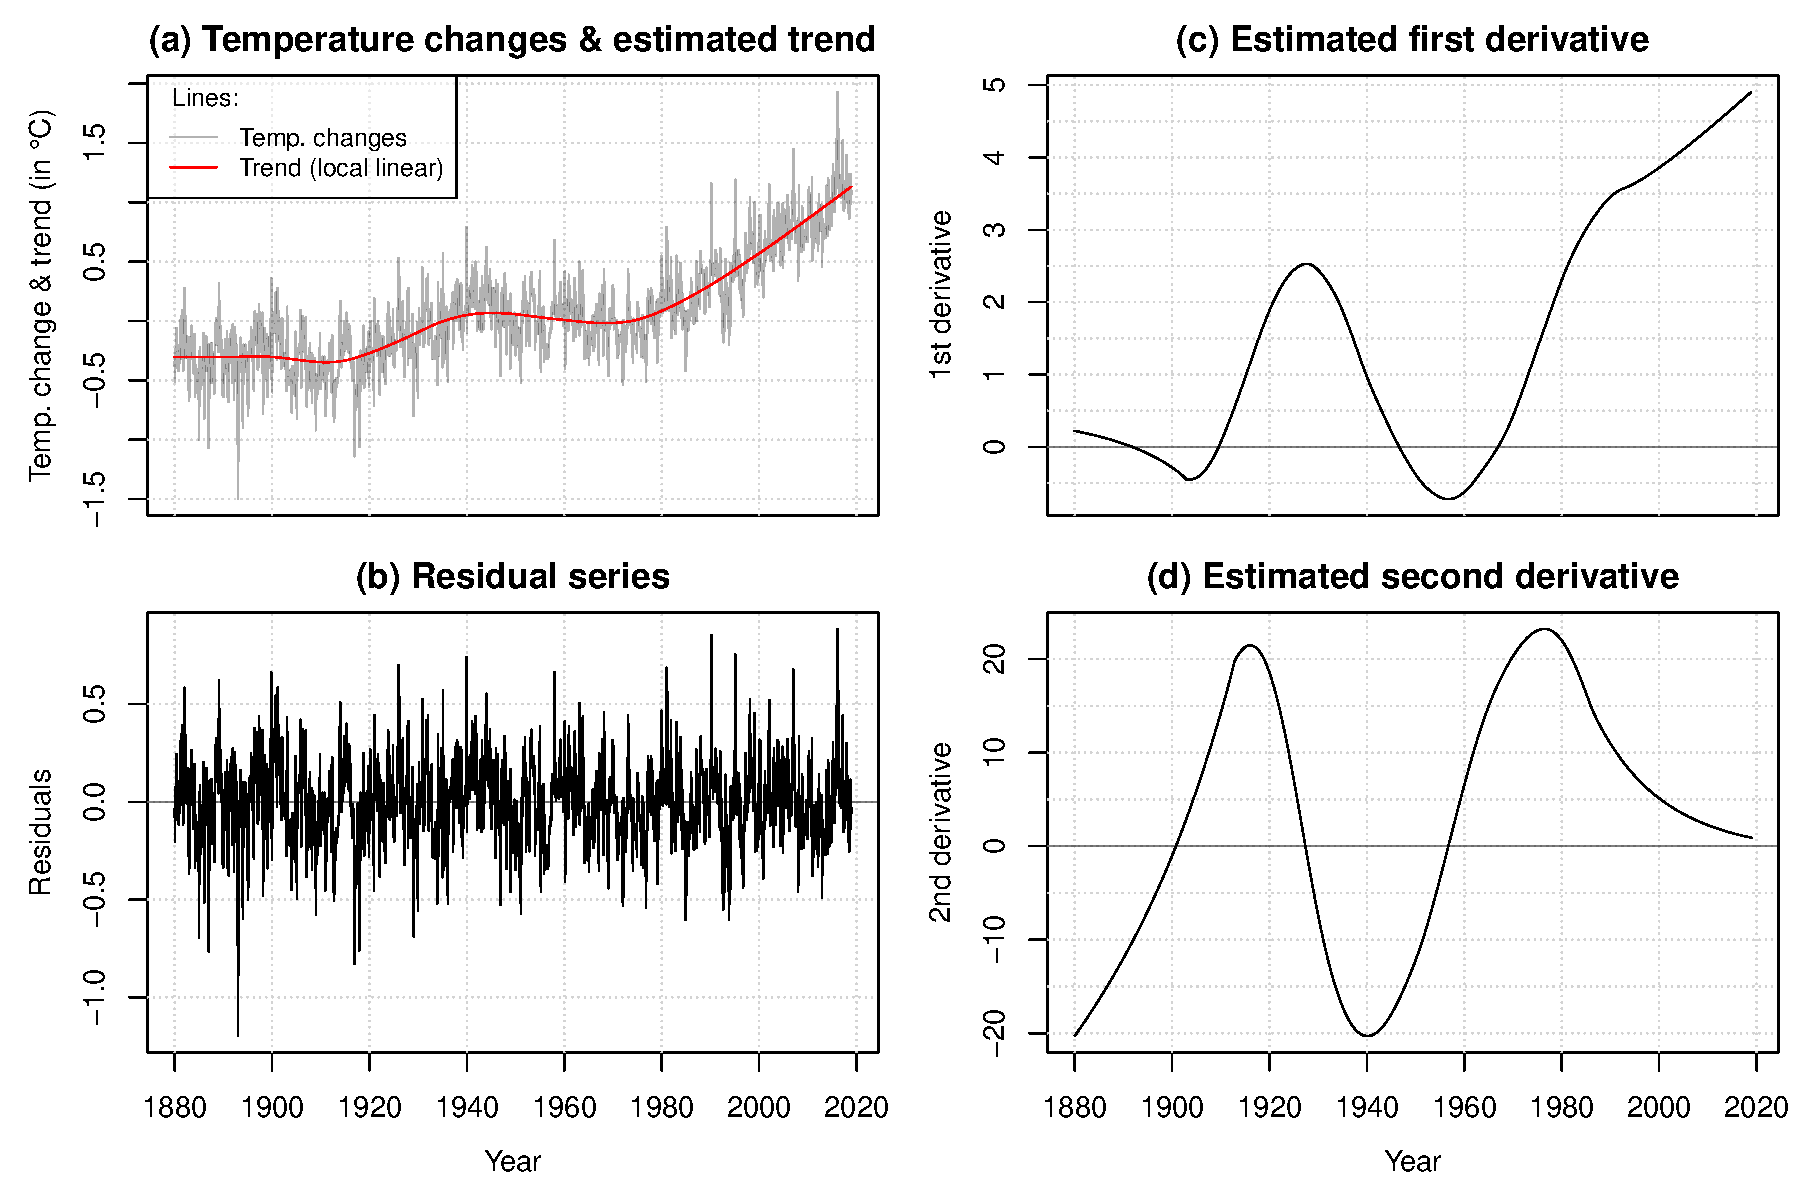
\includegraphics[width=\textwidth]
		{Plot1_TempChange_final.pdf}}
	\caption{\label{fig:ex1} The NHTM series and the estimated trend are displayed in (a). The residuals, as well as the estimated first and second derivatives are shown in (b), (c) and (d), respectively.}
\end{figure}

\subsection{A semiparametric log-local-linear growth model}

A well-known approach in developing economics is the log-linear growth model. Assume that the log-transformation of a macroeconomic time series follows Models \eqref{eq:Semi-MTS} and \eqref{eq:Semi-ARMA}, we achieve a semiparametric local polynomial, in particular a local-linear extension of this theory. To show this application, the series of the quarterly US-GDP from the first quarter of 1947 to the second quarter of 2019, downloaded from the Federal Reserve Bank of St. Louis, is chosen. Data-driven local linear regression is applied to estimate the trend from the log-data using \textit{AlgA} with the selected bandwidth 0.1325.
A kernel regression estimate using the same bandwidth is also carried out for comparison. 
\begin{example}
  l_gdp <- log(smoots::gdpUS$GDP)  
  gdp_t1 <- smoots::msmooth(l_gdp, p = 1, mu = 1, bStart = 0.1, alg = "A", 
    method = "lpr")
  gdp_t2 <- smoots::msmooth(l_gdp, p = 1, mu = 1, bStart = 0.1, alg = "A", 
    method = "kr")
  gdp_d1 <- smoots::dsmooth(l_gdp, d = 1, mu = 1, pp = 1, bStart.p = 0.1, 
    bStart = 0.15)
  gdp_d2 <- smoots::dsmooth(l_gdp, d = 2, mu = 1, pp = 1, bStart.p = 0.1, 
    bStart = 0.2) 
\end{example}
The results together with the log-data are displayed in Figure~\ref{fig:ex2}(a). We see that the two trend estimates in the middle part coincide with each other. They differ from each other only at the boundary points and the kernel estimate is affected by a clear boundary problem. Thus, the local linear method should be used. Residuals of this estimate are shown in Figure~\ref{fig:ex2}(b). Again, the estimated first and second derivatives are given in Figures~\ref{fig:ex2}(c) and \ref{fig:ex2}(d), respectively, which help us to discover more detailed features of the economic development in the US. 
\begin{example}
  arma2 <- stats::arima(gdp_t1$res, order = c(1, 0, 1), include.mean = FALSE)
\end{example}
Furthermore, the following ARMA(1, 1) model is obtained from the residuals: 
\begin{equation} \label{eq:resultEx2}
\tilde{\xi}_{t} = 0.9079\tilde{\xi}_{t-1} + 0.2771\varepsilon_{t-1} + \varepsilon_{t}. 
\end{equation} 
\begin{figure}[htbp]
	\center{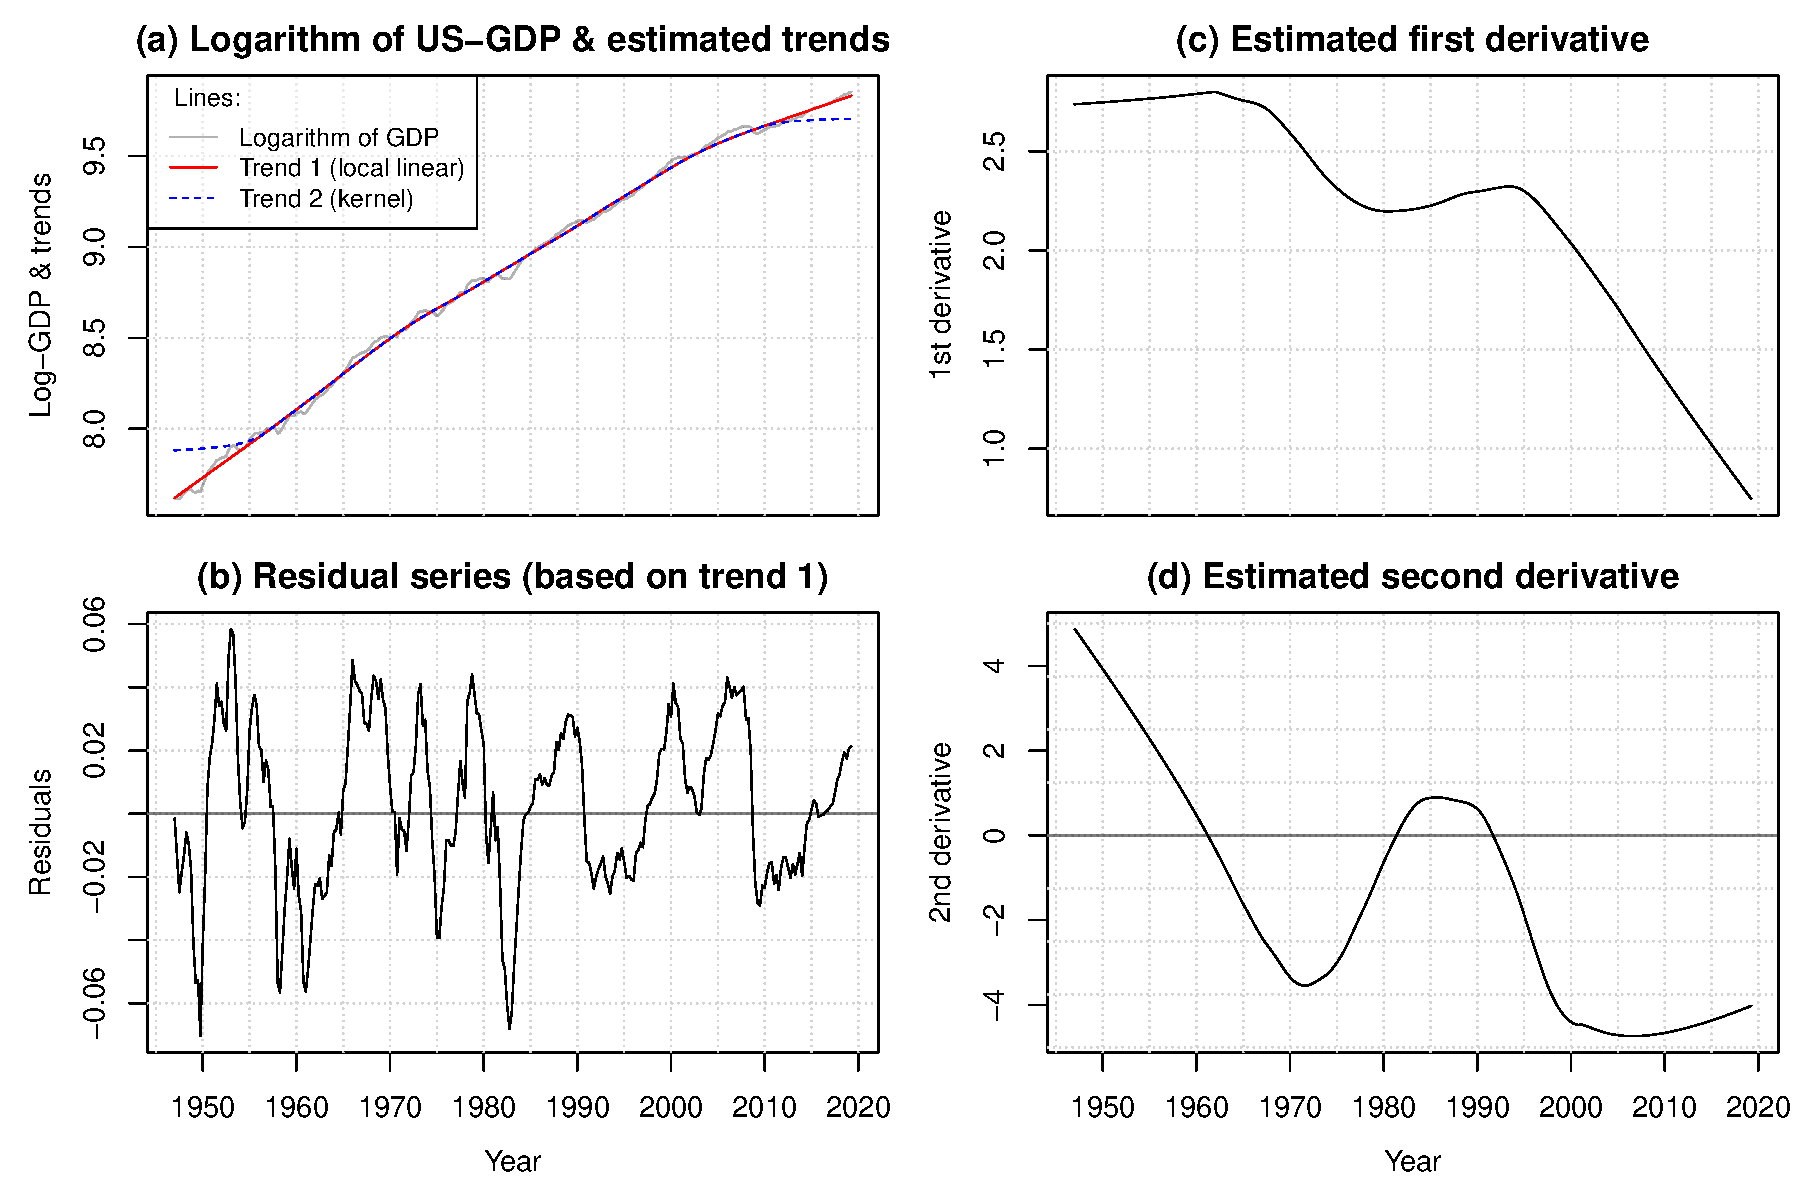
\includegraphics[width=\textwidth]
		{Plot2_GDP_final.pdf}}
	\caption{\label{fig:ex2} The log-transformed GDP series and the estimated trends are displayed in (a). The residuals based on the estimated local linear trend, as well as the estimated first and second derivatives are shown in (b), (c) and (d), respectively.}
\end{figure}

\section{The Semi-Log-GARCH model} \label{sec:SemiLogGARCH}

Most of the GARCH extensions, including the Log-GARCH \citep{pantula1986, geweke1986, milhoj1987multi}, are defined for stationary return series. Recently, \citet{francq2013garch} rediscovered the usefulness of the Log-GARCH.
In practice it is however found that the unconditional variance of financial returns may change slowly over time and are hence non-stationary. To overcome this problem a semiparametric GARCH (Semi-GARCH) approach is proposed by \citet{feng2004sim}, by defining the return series as a product of a (deterministic) smooth scale function and a GARCH model. 
Another well-known closely related approach is the Spline-GARCH introduced by \citet{engle2008spline}. In this paper we will introduce a Semi-Log-GARCH (semiparametric Log-GARCH), defined as a Log-GARCH with a smooth scale function. We propose to estimate the scale function in the Semi-Log-GARCH model based on the log-transformation of the squared returns as proposed by \citet{engle2008spline}.  

Denote the centralized returns by $r_t$, $t=1, ..., n$. The Semi-Log-GARCH model is defined by
\begin{equation} \label{eq:rt}
r_{t} = \sqrt{v\left(x_{t}\right)}\zeta_{t} \ \text{ with } \ \zeta_{t} = \sqrt{h_{t}}\eta_{t} \ \text{ and} 
\end{equation} 
\begin{equation} \label{eq:lnht}
\ln\left(h_{t}\right) = \omega + \sum_{i=1}^{l}\alpha_{i}\ln\left(\zeta_{t-i}^{2}\right) + \sum_{j=1}^{s}\beta_{j}\ln\left(h_{t-j}\right),
\end{equation}
where $v\left(x_{t}\right) > 0$ is a smooth local variance component, $h_t>0$ are conditional variances and $\eta_{t}$ are i.i.d. random variables with zero mean and unit variance. It is assumed that $\zeta_t$ also has unit variance and $\zeta_{t}\ne 0$ almost surely, so that the model is well-defined. 
Let $y_t=\ln\left(r_t^2\right)$,  $\xi_t=\ln\left(\zeta_t^2\right)-\mu_{lz}$ and $m\left(x_t\right)=\ln\left[v\left(x_t\right)\right] +\mu_{lz}$, where $\mu_{lz}=E\left[\ln\left(\zeta_t^2\right)\right]$. We see that the log-transformation of $r_t^2$ of the Semi-Log-GARCH model has the form $y_t=m\left(x_t\right)+\xi_t$, which is a special case of Model \eqref{eq:Semi-MTS}. Furthermore, define $\varepsilon_t=\ln\left(\eta_t^2\right)-\mu_{le}$ with $\mu_{le}=E\left[\ln\left(\eta_t^2\right)\right]$, which are i.i.d. zero mean innovations in the stationary process $\xi_t$. According to \cite{francq2018exponential}, $\xi_t$ has the following ARMA representation: 
\begin{equation}\label{eq:lgARMA}
\xi_t = \sum_{i=1}^{l^{*}}\varphi_{i}\xi_{t-i} + \sum_{j=1}^{s}\psi_{j}\varepsilon_{t-j} + \varepsilon_{t}  
\end{equation}
with $l^{*} = \text{max}(l, s)$. Thus, the Semi-Log-GARCH model is equivalent to a Semi-ARMA of the log-transformation of $r_t^2$ with the restriction that the AR order should not be less than the MA order. Hence, this model can be simply estimated using the \pkg{smoots} package and the \code{arima()} function of the \pkg{stats} package. To obtain the total volatilities $\sigma_t=\sqrt{v\left(x_{t}\right)h_{t}}$, we suggest to utilize the three-step estimation procedure as proposed in Section 3.3 of \citet{sucarrat2019log}, however, we recommend to explicitly conduct the auxiliary regression in Step 1 in \citet{sucarrat2019log} by using a data-driven local polynomial.
\begin{enumerate}
	\item[\enspace\enspace i)] Obtain estimates of the nonparametric trend function $\hat{m}\left(x_t\right)$ in $y_t$ via the \pkg{smoots} package.
	\item[\enspace ii)] Fit an ARMA($l^{*}, s$) model \eqref{eq:lgARMA} to the residuals $\tilde{\xi}_t=y_t-\hat{m}\left(x_t\right)$, for example with the \code{arima()} function of the \pkg{stats} package, and compute the ARMA residuals $\hat{\varepsilon}_t$.
	\item[iii)] Consider $\hat{\mu}_{le} = -\ln\left[\frac{1}{n}\sum_{i=1}^{n}\exp\left(\hat{\varepsilon}_i\right)\right]$ as an estimator of the log-moment $E\left[\ln\left(\eta_t^2\right)\right]$. Then the total volatilities are estimated as 
	\begin{equation} \label{eq:volEstimator}
	  \hat{\sigma}_t=\exp\left\{ \left[\tilde{\xi}_t - \hat{\varepsilon}_t + \hat{m}\left(x_t\right) - \hat{\mu}_{le}\right] / 2 \right\}.
	 \end{equation}
\end{enumerate}
Estimates of the conditional volatilities are also calculable similarly by following the same three-step procedure while replacing \eqref{eq:volEstimator} with $\sqrt{\hat{h}_t}=\exp\left[\left( \tilde{\xi}_t - \hat{\varepsilon}_t + \hat{\mu}_{lz} - \hat{\mu}_{le} \right)/2\right]$, where we suggest $\hat{\mu}_{lz}=-\ln\left[\frac{1}{n}\sum_{i=1}^{n}\exp\left(\tilde{\xi}_i\right)\right]$. 
An important characteristic of the illustrated estimation procedure is that explicit estimates of the Log-GARCH parameters $\omega$, $\alpha_i$, for $1 \leq i \leq p$, and $\beta_j$, for $1 \leq j \leq q$, are not required for computing $\hat{\sigma}_t$ or $\sqrt{\hat{h}_t}$ \citep{sucarrat2019log}. If, however, necessary, estimates could be derived by considering the relationships between the coefficients in \eqref{eq:lnht} and \eqref{eq:lgARMA}, which are $\alpha_i = \varphi_{i} + \psi_{i}$, $\beta_{j} = -\psi_{j}$, where the non-existing coefficients are assumed to be zero, and $\omega=\left(1-\sum_{i=1}^{l^{*}}\varphi_{i}\right)\mu_{lz}-\left(1+\sum_{j=1}^{s}\psi_{j}\right)\mu_{le}$.  
Note that the parametric part of the Semi-Log-GARCH can also be estimated directly using the R package \CRANpkg{lgarch} \citep{sucarrat2015lgarch}. Nonetheless, this approach will not be considered in the current paper.   

In the following, the DAX series from 1990 to July 2019 downloaded from Yahoo Finance is chosen to show the application of the Semi-Log-GARCH model. Note that an observed return can be sometimes exactly zero. To overcome this problem, the log-transformation is calculated for the squared centralized returns, which are a.s. non-zero. This would even be a necessary treatment, if the returns had a very small, but non-zero mean.  
\begin{example}
  # Calculate the centralized log-returns
  dax_close <- smoots::dax$Close; dax <- diff(log(dax_close))
  rt <- dax - mean(dax); yt <- log(rt ^ 2) 
\end{example}  
Subsequently, the previously described estimation procedure according to \citet{sucarrat2019log} is implemented by estimating the trend function in the logarithm of the squared returns \code{yt} with the function \code{msmooth()} of the \pkg{smoots} package. More specifically, a local cubic trend is fitted, while employing \emph{AlgA}.
\begin{example}
  # Step 1: Estimate the trend in the log-transformed data using 'smoots'                                    
  estim3 <- smoots::msmooth(yt, p = 3, alg = "A")
  m_xt <- estim3$ye

  # Step 2: Fit an ARMA model to the residuals	
  xi <- estim3$res
  arma3 <- arima(xi, order = c(1, 0, 1), include.mean = FALSE)

  # Step 3: Estimate further quantities and the total volatilities
  mu_le <- -log(mean(exp(arma3$residuals)))  
  vol <- exp((xi - arma3$residuals + m_xt - mu_le) / 2)
\end{example}
For reference, \code{estim3.2 <- \ smoots::msmooth(yt, \ p = 1, \ alg = "A")} is called, i.e. a local linear trend under consideration of \emph{AlgA} is estimated as well. The centralized log-returns and the log-transformed data with the two estimated trends (local linear: blue; local cubic: red) are displayed in Figures~\ref{fig:ex3}(a) and \ref{fig:ex3}(b). Moreover, the selected bandwidths are 0.0869 and 0.1013, respectively. Results in Figure~\ref{fig:ex3}(b) indicate that the unconditional variance of the DAX-returns changes slowly over time. Ultimately, the local cubic trend is chosen for further analysis, because here the results of the local linear approach are over-smoothed. 
The following ARMA(1, 1) model (see Step 2 in the code) is obtained from the residuals of the log-data
\begin{equation} \label{eq:resultEx3_1}
\tilde{\xi}_t = 0.9692\tilde{\xi}_{t-1} - 0.9221\varepsilon_{t-1} + \varepsilon_{t}\text{,} 
\end{equation}
whereas the re-transformed Log-GARCH(1, 1) formula is given by
\begin{equation} \label{eq:resultEx3_2}
\ln\left(h_{t}\right) = 0.0685 + 0.0471\ln\left(\zeta_{t-1}^{2}\right) + 0.9221 \ln\left(h_{t-1}\right) 
\end{equation}
following the idea of \citet{sucarrat2016log}. The estimated conditional volatility ($\sqrt{\hat h_t}$) and total volatility ($\hat{\sigma}_t$) series are displayed in Figures~\ref{fig:ex3}(c) and \ref{fig:ex3}(d).

\begin{figure}[H]
	\center{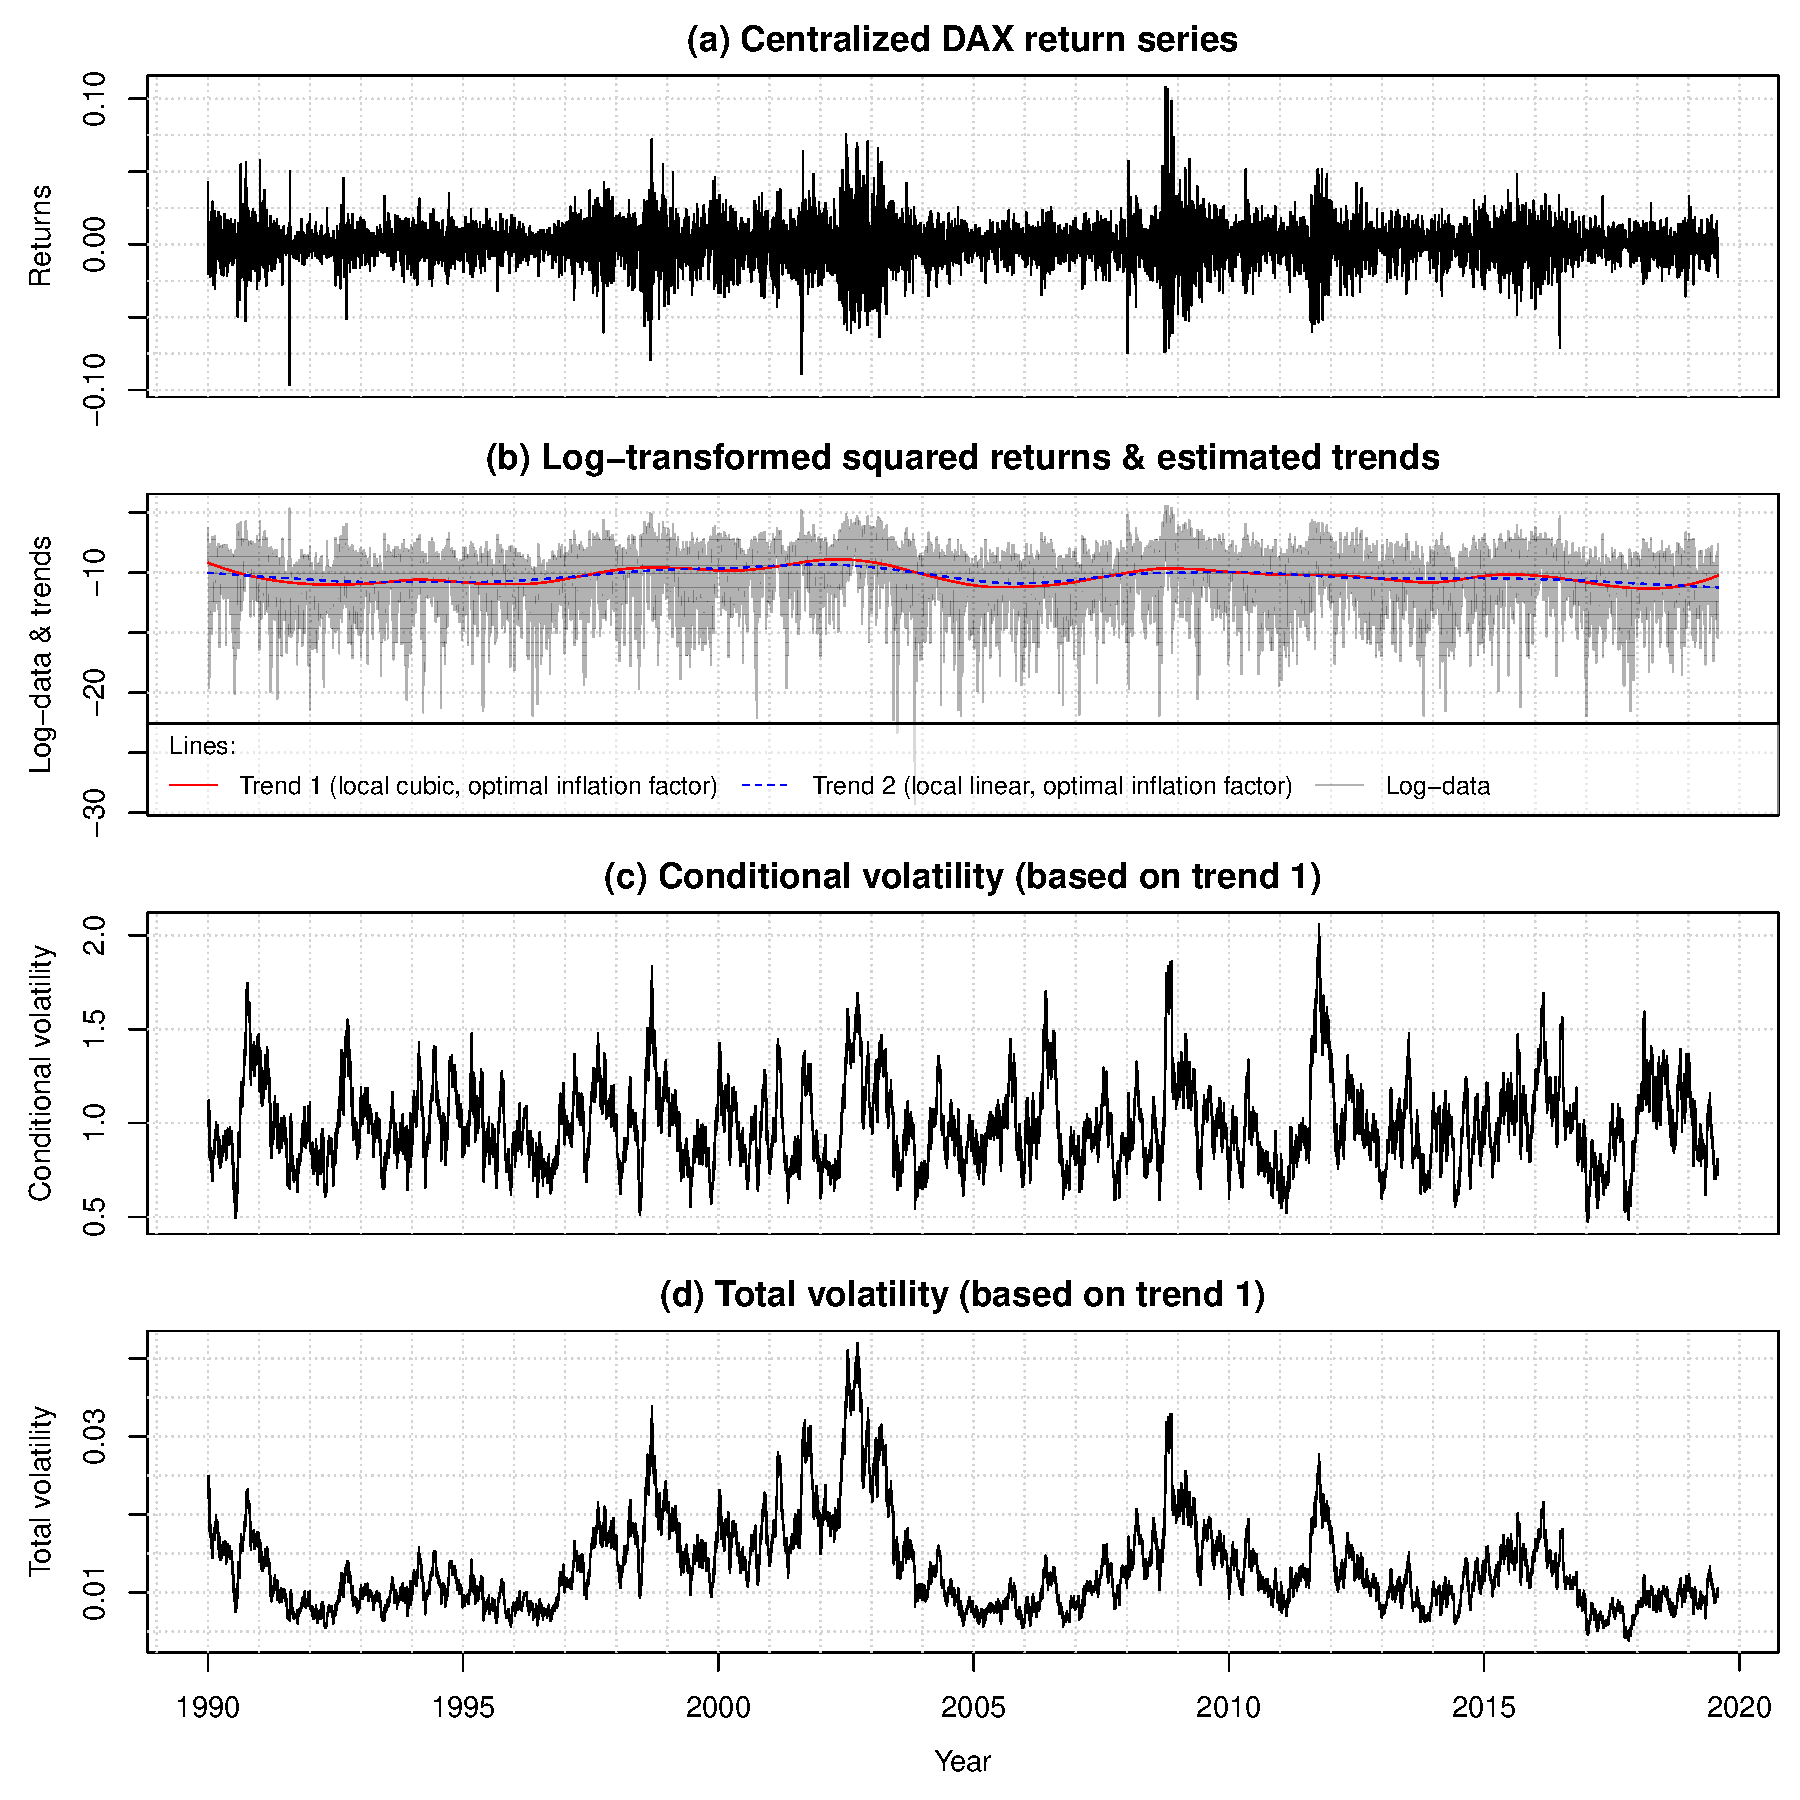
\includegraphics[width=\textwidth]
		{Plot3_DAX_final.pdf}}
	\caption{\label{fig:ex3} The demeaned DAX returns are displayed in (a). The log-transformed squared returns and the estimated trends are shown in (b). Based on the estimated local cubic trend, the corresponding estimated conditional and total volatilities are illustrated in (c) and (d), respectively.}
\end{figure}

\section{The Semi-Log-ACD model} \label{sec:SemiLogACD}

A more general framework for modeling non-negative financial time series is the ACD \citep[autoregressive conditional duration,][]{engle1998acd} model, which corresponds to a squared GARCH model and can be applied to both high-frequency or daily financial data. Logarithmic extensions of this approach were introduced by \citet{bauwens2000lacd}, where the Type I definition (called a Log-ACD) corresponds to a squared form of the Log-GARCH. Semiparametric generalization of the Log-ACD (Semi-Log-ACD) was defined and applied to different kinds of non-negative financial data by \citet{forstinger2018modelling}. 
In this paper, the application of the Semi-Log-ACD model will be illustrated by the CBOE Volatility Index (VIX) from 1990 to July 2019, denoted by $V_t$, $t=1, ..., n$. The data was again downloaded from Yahoo Finance. The Semi-Log-ACD model for $V_t$ is defined by
\begin{equation} \label{eq:SemiLogACD}
V_t=g\left(x_t\right) \lambda_t e_t, 
\end{equation} 
where $u_t=\lambda_t e_t$ follows a Log-ACD and $g\ge0$ is a smooth mean function in $V_t$, $\lambda_t\ge0$ is the conditional mean and $e_t$ is an i.i.d. series of non-negative random variables. It is assumed that $E\left(\lambda_t\right)=E\left(e_t\right)=1$. Further investigation on this model can be carried out similarly to that on the Semi-Log-GARCH model by replacing $r_t^2$, $h_t$ and $\eta_t^2$ there with $V_t$, $\lambda_t$ and $e_t$, respectively. 
The Semi-Log-ACD model can be similarly estimated. Discussion of those details is omitted. For further information we refer the reader to \citet{forstinger2018modelling} and references therein.	
\begin{example}
  # Calculate the logarithm of the index
  V <- smoots::vix$Close; lnV <- log(V)
\end{example}

\begin{figure}[H]
	\center{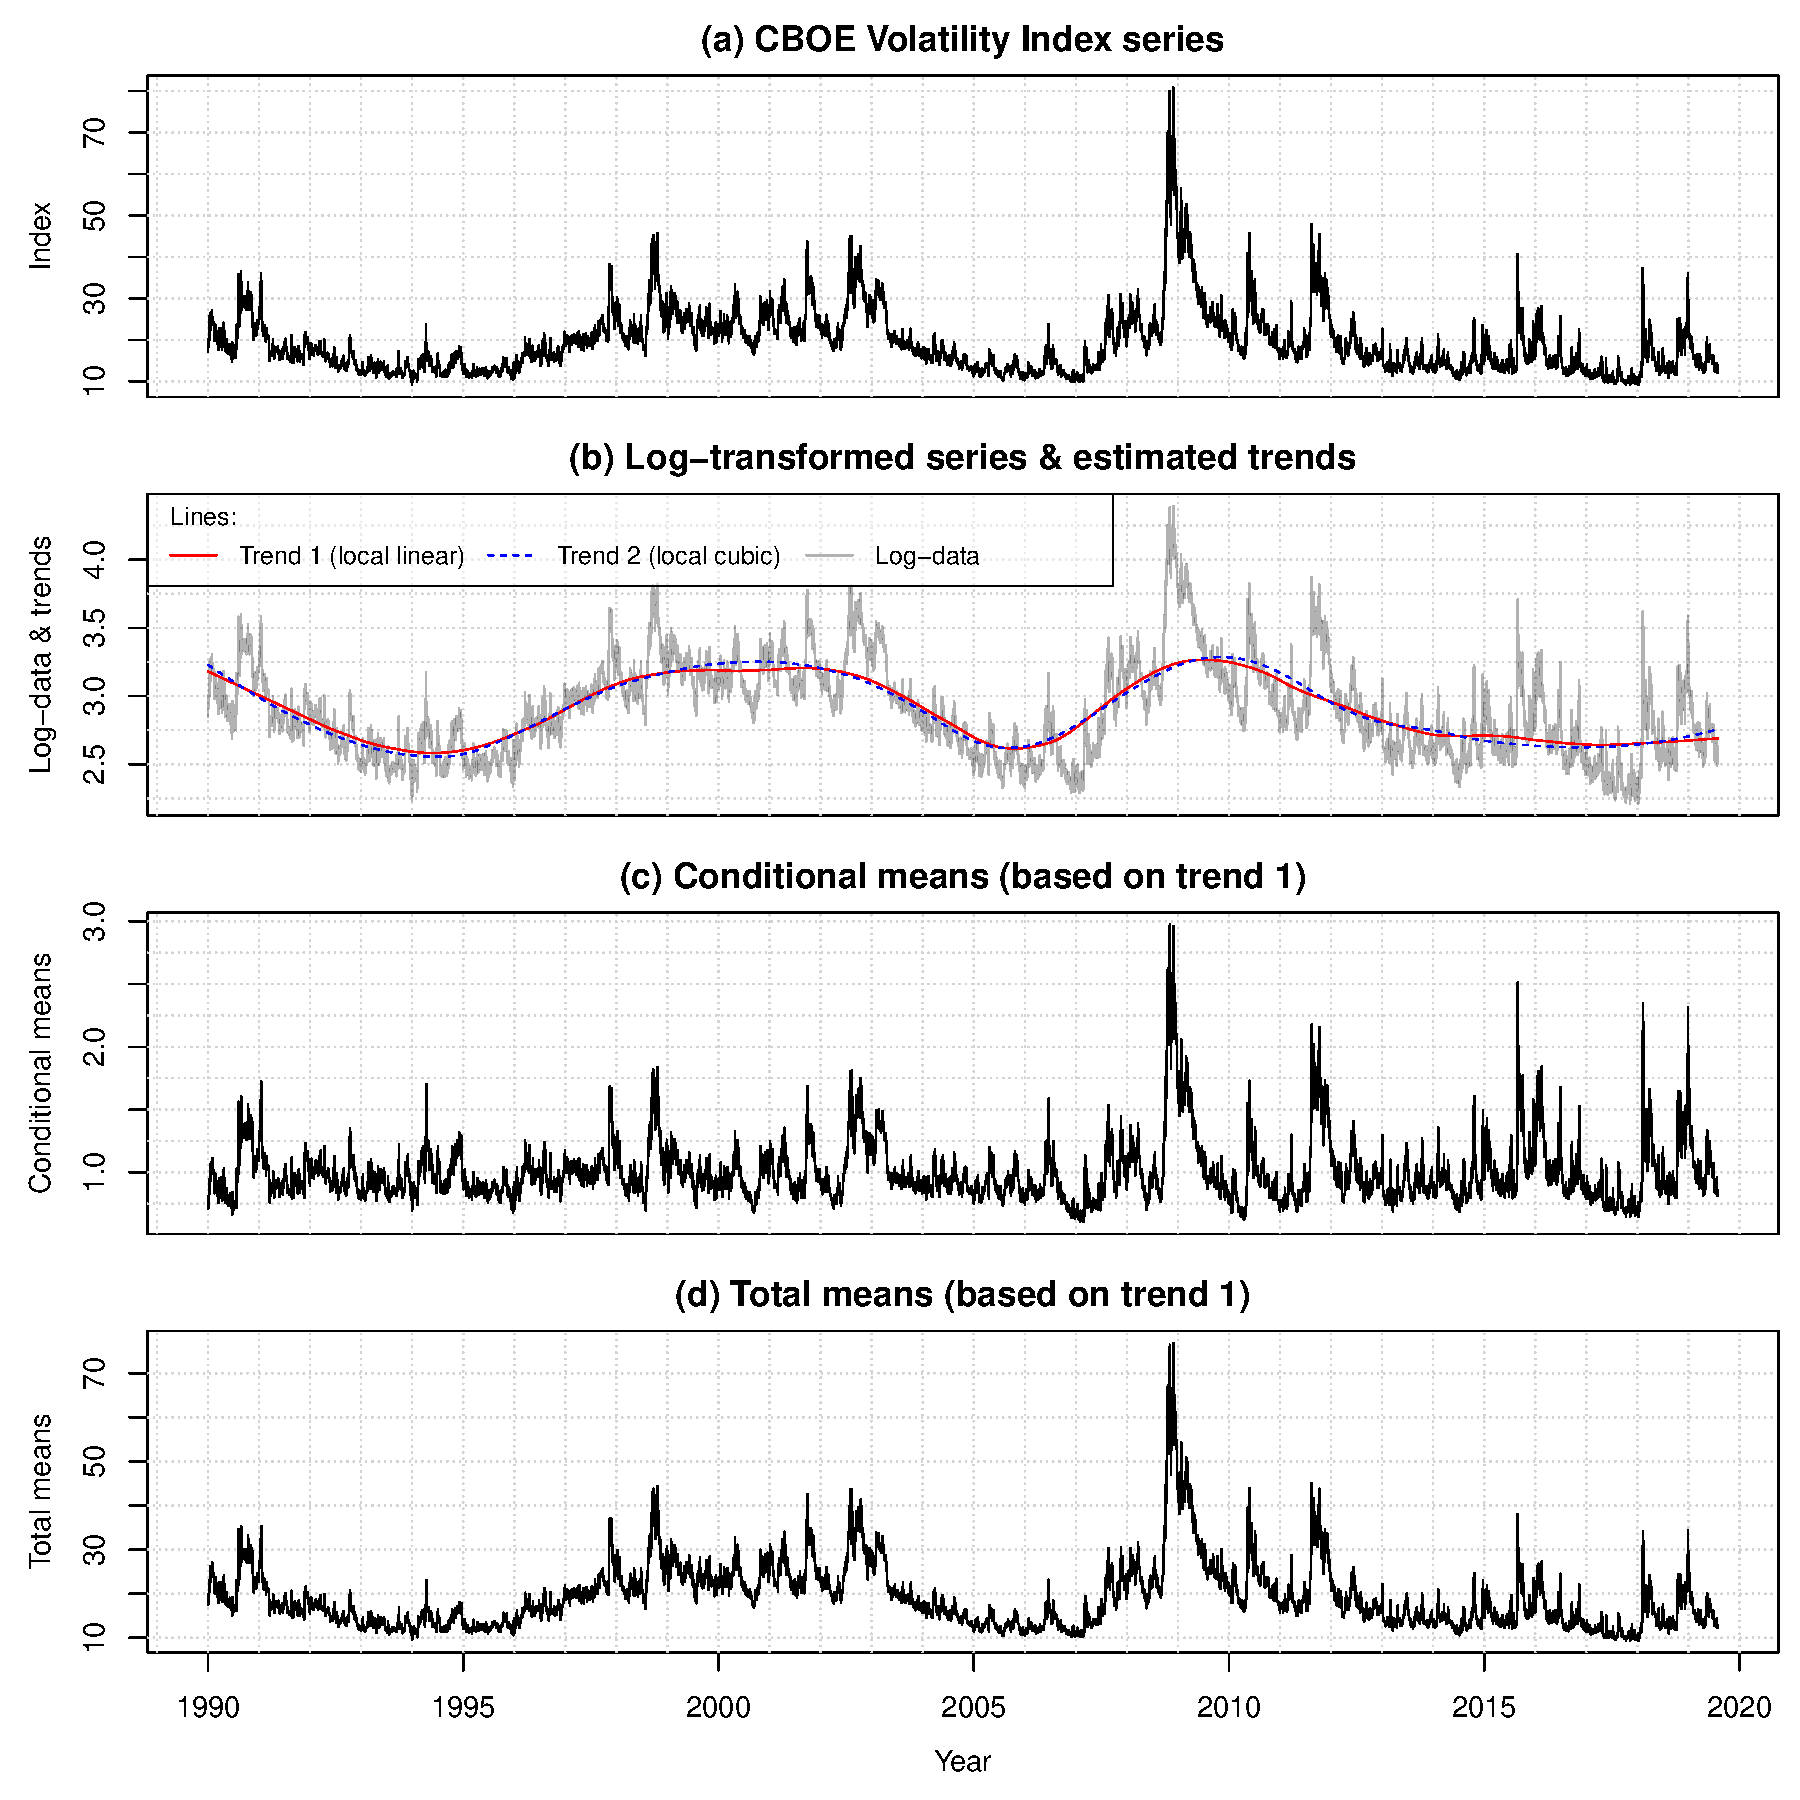
\includegraphics[width=\textwidth]
		{Plot4_VIX_final.pdf}}
	\caption{\label{fig:ex4} The VIX series is displayed in (a). The log-transformed index and the estimated trends are shown in (b). Based on the estimated local linear trend, the corresponding estimated conditional and total means are illustrated in (c) and (d), respectively.}
\end{figure}	

\begin{example}
  # Step 1: Estimate the trend in the log-transformed data using 'smoots'
  estim4 <- smoots::msmooth(lnV)
  estim4.2 <- smoots::msmooth(lnV, p = 3, alg = "B")
  m_xt <- estim4$ye

  # Step 2: Fit an ARMA model to the residuals
  xi <- estim4$res
  arma4 <- arima(xi, order = c(1, 0, 1), include.mean = FALSE) 
 
  # Step 3: Estimate further quantities and the total means 
  mu_le <- -log(mean(exp(arma4$residuals)))                             
  means <- exp(xi - arma4$residuals + m_xt - mu_le)                            
\end{example}
The original series of $V_t$ is shown in Figure~\ref{fig:ex4}(a). The trend was estimated from the log-transformation of $V_t$ using both \emph{AlgA} and \emph{AlgB} with the selected bandwidths 0.0771 and 0.1598, respectively. The data (black), the local linear trend (red) and the local cubic trend (blue) are displayed in Figure~\ref{fig:ex4}(b). The results using both algorithms are quite similar, except the local cubic estimates are smoother. From the residuals of the local linear approach the following ARMA(1, 1) model (see Step 2 in the code) is obtained: 
\begin{equation} \label{eq:resultEx4_1} 
\tilde{\xi}_{t} = 0.9626\tilde{\xi}_{t-1} - 0.0707\varepsilon_{t-1} + \varepsilon_{t}. 
\end{equation} 
Subsequently, the estimated log-form of the conditional mean function is given by 
\begin{equation} \label{eq:resultEx4_2}
\ln\left(\lambda_{t}\right) = 0.0010 + 0.8919\ln\left(u_{t-1}\right) + 0.0707\ln\left(\lambda_{t-1}\right). 
\end{equation} 
The estimated conditional means and the total means in the original data by the local linear approach are shown in Figures~\ref{fig:ex4}(c) and \ref{fig:ex4}(d). We see the results fit the data very well. This model can be applied for forecasting the VIX in the future.    

%\newpage

\section{Concluding remarks} \label{sec:conclusion}

In this paper the methodological background for developing the R package \pkg{smoots} (version 1.0.1) is summarized. The usage of the main functions in this package is explained in detail. To show the wide applicability of this approach two new semiparametric models for analyzing financial time series are also introduced. Data examples show that the proposed approach can be applied to different kinds non-stationary time series and the developed R package works very well for data-driven implementation of those semiparametric time series models. In particular, non-negative time series following a semiparametric multiplicative  
model can be easily estimated via the log-transformation. It is found that the errors in some examples could exhibit clear long memory. However, the current package is developed under short memory assumption. It is hence worthy to study the possible extension of the current approach to semiparametric time series models with long memory errors. Further extensions of the proposals in this paper, such as the development of suitable forecasting procedures and tools for testing stationarity of the errors or linearity of the deterministic trend, should also be studied in the future and included in future versions of the \pkg{smoots} package.

\section{Computational details} \label{optsec:CompDetails}

The numerical results in this paper were obtained using
R~4.1.1 with the
\pkg{smoots}~1.0.1 package and the \pkg{stats}~4.1.1 package. R itself
and all packages used are available from CRAN at \url{https://CRAN.R-project.org/}.

\vskip.5cm

\noindent{\bf Acknowledgments:} This work was supported by the German DFG project GZ-FE-1500-2-1. The data used were downloaded from different public sources as indicated in the contexts. We are grateful to the CRAN-network for great help during the publication of the R package \pkg{smoots}. 
We would also like to thank Dr. Marlon Fritz for helpful discussions.  

\bibliography{feng-gries-letmathe-schulz}

\address{Yuanhua Feng\\
  Department of Economics\\
  Faculty of Business Administration and Economics\\
  Paderborn University\\
  Warburger Straße 100, 33098 Paderborn\\
  Germany\\
  \email{yuanhua.feng@uni-paderborn.de}}

\address{Thomas Gries\\
  Department of Economics\\
  Faculty of Business Administration and Economics\\
  Paderborn University\\
  Warburger Straße 100, 33098 Paderborn\\
  Germany\\
  \email{thomas.gries@uni-paderborn.de}}

\address{Sebastian Letmathe\\
  Department of Economics\\
  Faculty of Business Administration and Economics\\
  Paderborn University\\
  Warburger Straße 100, 33098 Paderborn\\
  Germany\\
  \email{sebastian.letmathe@uni-paderborn.de}}

\address{Dominik Schulz\\
	Department of Economics\\
	Faculty of Business Administration and Economics\\
	Paderborn University\\
	Warburger Straße 100, 33098 Paderborn\\
	Germany\\
	\email{dominik.schulz@uni-paderborn.de}}